% arara: pdflatex: {interaction: nonstopmode, synctex: on,  shell: yes}
% arara: bibtex if found('log', 'Citation .* undefined')
% arara: pdflatex: {interaction: nonstopmode, synctex: on,  shell: yes}  if found('log', 'undefined references') or found('log', 'Rerun to') or found('log', 'Citation .* undefined')
% arara: pdflatex: {interaction: nonstopmode, synctex: on,  shell: yes}  if found('log', 'Rerun to') or found('log', 'Citation .* undefined')

\documentclass{cubeamer}
\input macros.tex
\input tikz.tex
\input acronyms.tex
\usetikzlibrary{positioning}
%%% Custom TikZ addons
\usetikzlibrary{crypto.symbols}
%\tikzset{shadows=no}  
\usetikzlibrary{decorations.pathreplacing}
\usetikzlibrary{arrows}
\usetikzlibrary{arrows.meta, fit, backgrounds}
\usetikzlibrary{patterns}
\usetikzlibrary{shapes}
\usetikzlibrary{shadows}
\usetikzlibrary{calc}
\usetikzlibrary{math}

\hypersetup{
    colorlinks=true,
    linkcolor=blue,
    citecolor=green,
    urlcolor=cyan
}
\def\makethanks{%
    \begin{frame}
        \frametitle{\thankstitle}
        \thanksmessage
    \end{frame}
}
% in ``article'' mode there's no ``Thank you'' page
\mode<article>
{\providecommand\makethanks{}}


% commands for the title and message of the "Thank you" page
\def\thankstitle#1{\def\thankstitle{#1}}
\def\thanksmessage#1{\def\thanksmessage{#1}}
\thankstitle{}
\thanksmessage{{\huge {\color{red} Thank You} for your attention!} \\ \Large Any questions?}


\title[Some Classical Attacks]{Some Classical Attacks}
% \subtitle{\green{National Workshop on Cryptology 2025, IIT Bhilai}}
\author[\red{Shibam}]{\red{Shibam Ghosh}$^1$}
\date{\today} % or whatever the date you are presenting in is
\institute[IIT Hyderabad]{$^1$\textcolor{redd}{Department of CSE, IIT Hyderabad}}
% \institute[INRIA, Paris]{INRIA, Paris, France}

 \AtBeginSection[] { %
    \begin{frame}[noframenumbering]
        \frametitle{Plan of this Section}
        \tableofcontents[
        currentsection,
        currentsubsection,
        sectionstyle=show/shaded,
        subsectionstyle=show/show/hide,
        subsubsectionstyle=hide]
    \end{frame}
}

% --- Frametitle Customization ---
\tcbuselibrary{many}
% \usepackage[many]{tcolorbox}
\setbeamertemplate{itemize item}{$\blacktriangleright$}
\setbeamertemplate{itemize subitem}{$\triangleright$}
\setbeamertemplate{itemize subsubitem}{$\rhd$}

% Later, reload hyperref with your desired options:
\hypersetup{
    colorlinks=true,
    linkcolor=blue,
    citecolor=green,
    urlcolor=cyan
}

% -------------------------------------------------------
% Define Cyan Color for Title
% -------------------------------------------------------
\definecolor{myctyan}{RGB}{0,180,200}
\definecolor{mytheme}{RGB}{0, 51, 102}
\definecolor{cardbg}{RGB}{235, 242, 252}  % Light blue tint
% -------------------------------------------------------
% Override Frame Title Template
% -------------------------------------------------------
\setbeamertemplate{frametitle}{
    \vspace{0.1cm}
    \textcolor{mytheme}{\Large\textbf{\insertframetitle}}
    \vspace{0.05cm}
}

% -------------------------------------------------------
% Remove Navigation Symbols
% -------------------------------------------------------
\setbeamertemplate{navigation symbols}{}

% -------------------------------------------------------
% Optional: Clean Footline
% -------------------------------------------------------
\setbeamertemplate{footline}{
    \begin{beamercolorbox}[wd=\paperwidth,ht=0.2cm,dp=0.2cm]{footline}
        \hspace{0.2cm}
        
\includegraphics[scale=0.03]{img/iith.png}
        \hfill
        \textcolor{gray}{\tiny\insertframenumber\,/\,\inserttotalframenumber}
        \hspace{0.5cm}
    \end{beamercolorbox}
}

% ---- ADD THIS AT THE END OF YOUR PREAMBLE ----
\makeatletter
\beamer@frametopskip=0pt plus 0pt\relax       % No flexible space on top
\beamer@framebottomskip=0pt plus 1fill\relax  % All flexible space goes to bottom
\makeatother


\usepackage{etoolbox}
\makeatletter
% Remove top filler from frame body
\patchcmd{\beamer@calculateheadfoot}{\vfill}{}{}{}
\makeatother
% ----------------------------------------------

% Put this in your preamble

% Section slide
\AtBeginSection[]{
    \begin{frame}[plain, noframenumbering]
        \begin{center}
            \vfill
            \textcolor{myctyan}{\rule{0.6\textwidth}{1.5pt}}
            \vspace{0.3cm}

            \textcolor{myctyan}{\Huge\textbf{\insertsectionhead}}

            \vspace{0.3cm}
            \textcolor{myctyan}{\rule{0.6\textwidth}{1.5pt}}
            \vfill
        \end{center}
    \end{frame}
}

% Subsection slide
\AtBeginSubsection[]{
    \begin{frame}[plain, noframenumbering]
        \begin{center}
            \vfill

            % Show parent section in smaller text above
            \textcolor{myctyan!60}{\large\textbf{\insertsectionhead}}

            \vspace{0.3cm}
            \textcolor{myctyan}{\rule{0.4\textwidth}{0.8pt}}
            \vspace{0.3cm}

            % Show subsection in larger text below
            \textcolor{myctyan}{\LARGE\textbf{\insertsubsectionhead}}

            \vfill
        \end{center}
    \end{frame}
}

\newcommand{\h}{\ensuremath{\mathcal{H}}}
% --- Corrected TikZ styles using the modern \tikzset syntax ---
\tikzset{
    block/.style = {draw, rectangle, minimum height=1cm, minimum width=1cm, thick},
    xor/.style   = {draw, circle, thick, inner sep=0pt, minimum size=4mm},
    data/.style  = {font=\Large\ttfamily}
}

\tikzset{
    % Your custom style, named 'bigblock'
    bigblock/.style={
        fill=blue!10,
        rectangle,
        draw=violet,
        semithick,
        inner sep=5pt,      % NOTE: I set this to 5pt. 0pt makes the text touch the border.
        minimum height=1cm,
        minimum width=1.5cm,  % NOTE: I set this to 1.5cm to comfortably fit "E_a".
        rounded corners=1mm,
    },
    % Other styles from the previous version
    blockdata/.style  = {draw, rectangle, minimum size=1.2cm, thick, fill=gray!10, font=\large\ttfamily},
    key/.style   = {font=\small\ttfamily, fill=red!10, draw, rounded corners},
    middle/.style = {draw, rectangle, rounded corners, minimum height=1.2cm, minimum width=1.5cm, thick, fill=green!15, font=\large\ttfamily},
    arrow/.style = {-{Stealth[length=2.5mm]}, thick}
}


% --- A REUSABLE COMMAND FOR THE FEISTEL DIAGRAM (WITH EXPLICIT SWAP) ---
\newcommand{\feisteldiagram}{%
    \centering
    % The >={...} option sets the default arrowhead for all paths drawn with ->
    \begin{tikzpicture}[
        node distance=1.5cm,
        >={Stealth[length=2mm]} 
    ]

        % Place inputs
        \node[data] (L0) at (0,0) {$L_i$};
        \node[data] (R0) at (3,0) {$R_i$};
        
        % Place the F function and XOR at the middle level
        \coordinate (midlevel) at (0, -2);
        \node[bigblock] (F) at ($(L0)!0.5!(R0) + (midlevel)$) {$F$};
        \node[xor] (XOR) at (F -| L0) {\Large $\oplus$};
        
        % Key input (moved slightly for better spacing)
        \node[key, above=1cm of F] (Ki) {$K_{i}$};

        % Place outputs (in their final, NON-swapped positions)
        \coordinate (semifinallevel) at (0, -3);
        \coordinate (Li11) at (semifinallevel -| L0);
        \coordinate (Ri11) at (semifinallevel -| R0);

        % Place outputs (in their final, NON-swapped positions)
        \coordinate (finallevel) at (0, -5);
        \node[data] (Li1) at (finallevel -| L0) {$L_{i+1}$};
        \node[data] (Ri1) at (finallevel -| R0) {$R_{i+1}$};

        % --- Draw the paths using -> to apply the default arrowhead ---
        % Core round function paths
        \draw[->] (L0.south) -- (XOR);
        \draw[->] (F) -- (XOR);
        \draw[arrow, dashed] (Ki) -- (F);


        % --- The right-hand path and the EXPLICIT SWAP ---
        % Define the corner where the right path turns to go to F
        \coordinate (turnpoint) at (R0 |- F);
        % Draw the vertical line from R_i to the turn point (no arrow)
        \draw (R0.south) -- (turnpoint);
        % Draw the horizontal line from the turn point into F (with arrow)
        \draw[->] (turnpoint) -- (F);
        
        \draw[-] (XOR) -- (Li11);
        \draw[-] (turnpoint) -- (Ri11);

        % --- Draw the CROSSING/SWAP lines ---
        % The right branch becomes the new Left branch
        \draw[->] (Ri11) -- (Li1);
        % The left (XORed) branch becomes the new Right branch
        \draw[->] (Li11) -- (Ri1);
    \end{tikzpicture}%
}

\begin{document}

\maketitle

\begin{frame}[t]
    \frametitle{Table of contents}
    \tableofcontents
\end{frame}
%\cutoc

\section{The Round Function of a Feistel Structure}
% --- SLIDE 2: The Feistel Structure (Visual + Math) ---
\begin{frame}
    \frametitle{The Feistel Structure}
    \begin{columns}[c] % Vertically centered columns
        \begin{column}{0.3\textwidth}
            \feisteldiagram % Use our new command
        \end{column}
        
        \begin{column}{0.6\textwidth}
            \begin{block}{Encryption Round}
                \begin{align*}
                    L_{i+1} &= R_i \\
                    R_{i+1} &= L_i \oplus F(K_{i}, R_i)
                \end{align*}
            \end{block}
        \end{column}
    \end{columns}
\end{frame}

% --- SLIDE 3: Case 1 ---
\begin{frame}[fragile]
    \frametitle{Exploring Weak Functions}
    \begin{columns}[T] % Top-aligned columns
        \begin{column}{0.5\textwidth}
            \feisteldiagram % The diagram remains
        \end{column}
        
        \begin{column}{0.5\textwidth}
            \begin{block}{Case 1: The Zero Function}
                What if $F(K, x) = 0 \forall x$?
            \end{block}
            
            \pause
            
            \uncover<2->{$
            \begin{aligned}[t]
                L_1 &= R_0 \\ R_1 &= L_0 \oplus 0 = L_0 \\
            \end{aligned}
            $}

            \uncover<3->{$
            \begin{aligned}[t]
                L_2 &= L_0  \\ R_2 &= R_0 \\
            \end{aligned}
            $}

            \uncover<4->{
            \begin{alertblock}{Result}
                After an even number of rounds, you get the input back. \red{No security!}
            \end{alertblock}}
        \end{column}
    \end{columns}
\end{frame}

% --- SLIDE 4: Case 2 ---
\begin{frame}[fragile]
    \frametitle{Exploring Weak Functions}
    \begin{columns}[T]
        \begin{column}{0.5\textwidth}
            \feisteldiagram % The diagram remains
        \end{column}
        
        \begin{column}{0.5\textwidth}
            \begin{block}{Case 2: The Identity Function}
                What if $F(K, x) = x, \forall x$?
            \end{block}
            
            \uncover<2->{$
            \begin{aligned}[t]
                L_1 &= R_0 \\ R_1 &= L_0 \oplus R_0 \\
            \end{aligned}
            $}

            \uncover<3->{$
            \begin{aligned}[t]
                L_2 &= L_0 \oplus R_0 \\ R_2 &= R_0 \oplus (L_0 \oplus R_0) = L_0 \\
            \end{aligned}
            $}
            
            \uncover<4->{$
            \begin{aligned}[t]
                L_3 &= L_0 \\ R_3 &= (L_0 \oplus R_0) \oplus L_0 = R_0
            \end{aligned}
            $}
            
            \uncover<4->{
            \begin{alertblock}{Result}
                The input $(L_0, R_0)$ is restored after just 3 rounds. \red{No security!}
            \end{alertblock}}
        \end{column}
    \end{columns}
\end{frame}

% --- SLIDE 5: Case 3 ---
\begin{frame}[fragile]
    \frametitle{Exploring Weak Functions}
    \begin{columns}[T]
        \begin{column}{0.5\textwidth}
            \feisteldiagram % The diagram remains
        \end{column}
        
        \begin{column}{0.5\textwidth}
            \begin{block}{Case 3: Simple XOR with Key}
                What if $F(K, x) = K \oplus x \forall x$?
            \end{block}
            
            \pause
            \uncover<2->{$
            \begin{aligned}[t]
                L_1 &= R_0 \\
                R_1 &= L_0 \oplus R_0 \oplus K_1 \\
            \end{aligned}
            $}
            \uncover<3->{$
            \begin{aligned}[t]
                L_2 &= L_0 \oplus R_0 \oplus K_1 \\
                R_2 &= R_0 \oplus (L_0 \oplus L_2) \oplus K_2 \\
                   &= L_0 \oplus K_1 \oplus K_2
            \end{aligned}
            $}

            \pause
            
            \uncover<3->{
            \begin{alertblock}{Result}
                The output is just a linear function of the input and keys. Broken with basic algebra. \red{No security!}
            \end{alertblock}}
        \end{column}
    \end{columns}
\end{frame}

% --- SLIDE 6: Conclusion (No diagram needed here) ---
\begin{frame}
    \frametitle{Conclusion: The Round Function is Everything}
    
    \begin{block}{Main Lesson}
        A Feistel network is excellent \textbf{structure}, but its \textbf{round function} is everything.
    \end{block}
    
    \begin{itemize}
        \item<2-> Weak or simple $F$ functions lead to ciphers that are trivially broken.
        \item<3-> A strong $F$ function must be \textbf{non-linear}
    \end{itemize}
    
\end{frame}

\section{Meet-in-the-middle}

% --- SLIDE 2: Visualizing Double Encryption (The Forward Path) ---
\begin{frame}
    \frametitle{Double Encryption}
    
    \begin{center}
    \begin{tikzpicture}[node distance=1cm]
        % Nodes
        \node[data] (p) {$p$};
        \node[bigblock, right=of p] (Ea) {$E^a$}; % Applied 'bigblock' style
        \node[data, right=of Ea] (m) {$m$};
        \node[bigblock, right=of m] (Eb) {$E^b$}; % Applied 'bigblock' style
        \node[data, right=of Eb] (c) {$c$};
        \node[key, above=1cm of Ea] (k1) {$K_1$};
        \node[key, above=1cm of Eb] (k2) {$K_2$};
        
        % Arrows
        \draw[arrow] (p) -- (Ea);
        \draw[arrow] (Ea) -- (m);
        \draw[arrow] (m) -- (Eb);
        \draw[arrow] (Eb) -- (c);
        \draw[arrow, dashed] (k1) -- (Ea);
        \draw[arrow, dashed] (k2) -- (Eb);
    \end{tikzpicture}
    \end{center}
    The Encryption Process:
    \(c = E^b(K_2, \underbrace{E^a(K_1, p)}_{m}), \text{ where master-key }K = (K_1, K_2) \)
\pause
   \begin{center}
    \begin{tikzpicture}[node distance=1cm]
        % Nodes
        \node[data] (p) {$p$};
        \node[bigblock, right=of p] (Da) {$D^a$}; % Applied 'bigblock' style
        \node[middle, right=of Da] (m) {$m$};
        \node[bigblock, right=of m] (Db) {$D^b$}; % Applied 'bigblock' style
        \node[data, right=of Db] (c) {$c$};
        \node[key, above=1cm of Da] (k1) {$K_1$};
        \node[key, above=1cm of Db] (k2) {$K_2$};
        
        % Arrows (in reverse)
        \draw[arrow] (c) -- (Db);
        \draw[arrow] (Db) -- (m);
        \draw[arrow] (m) -- (Da);
        \draw[arrow] (Da) -- (p);
        \draw[arrow, dashed] (k2) -- (Db);
        \draw[arrow, dashed] (k1) -- (Da);
    \end{tikzpicture}
    \end{center}

\end{frame}

% --- SLIDE: The Core Meet-in-the-Middle Condition ---
\begin{frame}
    \frametitle{The Filtering Condition}
    
    \begin{center}
    \begin{tikzpicture}[
        key_box/.style={draw=red, thick, rectangle, rounded corners, fill=red!10, font=\large\ttfamily},
    ]
    
        % --- The single, unknown key pair we are looking for ---
        \node[key_box] (K) at (0, 1.5) {$(K_1, K_2)$};
    
        % --- The known plaintext/ciphertext pairs ---
        \node[data] (p1) at (-4, 0) {$p_1$};
        \node[data] (c1) at (4, 0)  {$c_1$};
        \node[middle] (m1) at (0, 0) {$m_1$};
        
        \uncover<2->{
        \node[data] (p2) at (-4, -2) {$p_2$};
        \node[data] (c2) at (4, -2)  {$c_2$};
        \node[middle] (m2) at (0, -2) {$m_2$};

        \node[font=\Large] at (-4, -3.2) {$\vdots$};
        \node[font=\Large] at (4, -3.2) {$\vdots$};
        \node[font=\Large] at (0, -3.2) {$\vdots$};
        }

        % --- The arrows representing the condition ---
        \draw[->, thick, blue] (p1) -- (m1) node[midway, above, font=\small] {$E^a$};
        \draw[<-, thick, red] (c1) -- (m1) node[midway, above, font=\small] {$D^b$};

        \uncover<2->{
        \draw[->, thick, blue] (p2) -- (m2) node[midway, above, font=\small] {$E^a$};
        \draw[<-, thick, red] (c2) -- (m2) node[midway, above, font=\small] {$D^b$};
        }
        
        % --- Dashed lines showing the key's influence ---
        \draw[->, dashed, red!80] (K) to[bend right=15] (p1.north);
        \draw[->, dashed, red!80] (K) to[bend left=15] (c1.north);
        \uncover<2->{
        \draw[->, dashed, red!80] (K) to[bend right=10] (p2.north);
        \draw[->, dashed, red!80] (K) to[bend left=10] (c2.north);
        }

    \end{tikzpicture}
    
    \uncover<3->{
        The Constraint: \(E^a(K_1, p_i) = \red{m_i} = D^b(K_2, c_i) \quad \text{for all } i=1, 2, \dots, t\)
    }

    \end{center}
\end{frame}

% --- SLIDE: The Meet-in-the-Middle Algorithm (FINAL CORRECTION) ---
% \begin{frame}
%     \frametitle{The Attack Algorithm in Action}
    
%     \begin{columns}[T] % Top-aligned columns
    
%         % --- LEFT COLUMN: Steps 1 & 2 ---
%         \begin{column}{0.5\textwidth}
%             \centering
%             \textbf{Step 1: Build Forward Table}
            
%             \begin{tikzpicture}[
%                 node distance=0.8cm,
%                 table_node/.style={draw, rectangle, fill=blue!5}
%             ]
%                 \node[data] (p) {$(p_1, c_1)$};
%                 \node[bigblock, below=of p] (Ea) {Encrypt with \\ all possible $k_a$};
                
%                 \uncover<2->{
%                 % The table T1
%                 \node[table_node, below=of Ea] (T1) {
%                     \small
%                     \begin{tabular}{c|c}
%                         \multicolumn{2}{c}{\textbf{Table $T_1$}} \\ \hline
%                         \textbf{Value} & \textbf{Key} \\ \hline
%                         $m_{a1}$ & $k_{a1}$ \\
%                         $m_{a2}$ & $k_{a2}$ \\
%                         \dots & \dots \\
%                         \uncover<5->{\tikz[overlay]{\node[fit=(mMatchNode)(kMatchNode), draw=red, thick, rounded corners] {};}}
%                         \node (mMatchNode) {$m_{ax}$}; & \node (kMatchNode) {$k_{ax}$}; \\
%                         \dots & \dots \\
%                         $m_{aN}$ & $k_{aN}$ \\
%                     \end{tabular}
%                 };
                
%                 \draw[arrow] (p) -- (Ea);
%                 \draw[arrow] (Ea) -- (T1);
%                 }
                
%                 \uncover<3->{
%                 \node[left=0.2cm of T1, draw, dashed, rounded corners, fill=yellow!20] (sort) {\textbf{Step 2: Sort $T_1$}};
%                 }
%             \end{tikzpicture}
%         \end{column}
        
%         % --- RIGHT COLUMN: Steps 3 & 4 ---
%         \begin{column}{0.5\textwidth}
%             \centering
%             \uncover<4->{
%             \textbf{Step 3: Search from Backward}
            
%             \begin{tikzpicture}[node distance=0.8cm]
%                 \node[data] (c) {$(p_1, c_1)$};
%                 \node[bigblock, below=of c] (Db) {For each $k_b$, \\ Decrypt $c_1$};
                
%                 % ***** THIS WAS THE LINE CAUSING THE ERROR *****
%                 % CORRECTED: The '*' must be inside math mode.
%                 \node[middle, below=of Db] (target) {Target Value $m^*$};
                
%                 \draw[arrow] (c) -- (Db);
%                 \draw[arrow] (Db) -- (target);
                
%                 \uncover<5->{
%                 \node[key_candidate, below=2cm of target] (candidate) {Candidate: $(k_{ax}, k_b)$};
%                 \draw[arrow, dashed] (Db) -- (candidate);
%                 }
%             \end{tikzpicture}
%             }
%         \end{column}
    
%     \end{columns}
    
%     % --- Arrow connecting the two sides ---
%     \uncover<5->{
%     \begin{tikzpicture}[overlay, remember picture]
%         \node (L) at (current page.west) {};
%         \node (R) at (current page.east) {};
        
%         \path (L) -- (R) node[midway, below=4cm] (searchLabelNode) {\textbf{Step 4: Find a Match}};
%         \draw[arrow, red, thick, bend right] 
%             (searchLabelNode.west -| R) ++(-4.5, 0.5)
%             to (searchLabelNode.east -| L) ++(4.5, 0.5);
%     \end{tikzpicture}
%     }
    
% \end{frame}

\begin{frame}
	\frametitle{Double encryption: Meet-in-the-middle}
	Consider a plaintext-ciphertext pair $(p_1,c_1)$.
	\begin{enumerate}
		\item Construct a table $T_1$ with rows of the form 
		$(c,k_a), \text{ where } E_a(k_a,p_1) = c.$
		\item Sort the table $T_1$ by first element.
		\item For every $k_b$, search for $D_b(k_b,c_1)$ in $T_1$.
		\item If there is a match and $k_a$ is the second element, then we have a candidate key $(k_a,k_b)$
	\end{enumerate}
	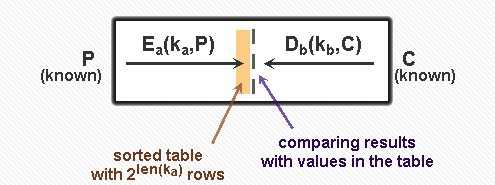
\includegraphics[width=0.8\textwidth]{./fig/meetinmi1.png}
\end{frame}

\begin{frame}
	\frametitle{Double Encryption: Meet-in-the-middle}
	\begin{block}{Complexity of the attack}
		Time complexity: $n2^{m}$\\
		Space complexity: $\ell 2^n$
		\begin{enumerate}
			\item $2^{m}:$ Compute $D_{k_b}$ for every $k_b$
			\item $n2^m:$ To sort the table $T_1$.
			\item $2^n(n+\ell):$ Size of the table $T_1$
		\end{enumerate}
	\end{block}
\end{frame}
\begin{frame}
	\frametitle{Double DES: Meet-in-the-middle}
	\begin{block}{}
	Meet-in-the-middle attack exploit the equation $E_a(k_1,p_i) = D_b(k_2,c_i)$ which holds for any $(p_i,c_i)$.\\
	What is the expected number of keys $(k_1,k_2)$ such that $E_a(k_1,p_i) = D_b(k_2,c_i)$ holds for $t$ pairs of $(p_i,c_i)$?
	\end{block}
	\begin{enumerate}
		\item Suppose we fix $p$ and choose a random $k_1$. Then $\Pr[E_a(k_1,p) = z] = 2^{-|k_1|}$ for all $z$.
		\item Similarly, if we fix $c$ and choose a random $k_2$. Then $\Pr[D_b(k_2,c) = z] = 2^{-|k_2|} = 2^{-|k_1|}$ for all $z$ (assume $|k_1| = |k_2|$).
		\item Thus $\Pr[E_a(k_1,p) = D_b(k_2,c)] = 2^{-|k_1|}$.
		\item If we consider $t$ pairs, then the above equation holds for all pairs with probability $2^{-t|k_1|}$.
		\item As there are total $2^{2|k_1|}$ possible keys, the expected number of keys is $2^{2|k_1|-t|k_1|}$.
	\end{enumerate}
\end{frame}
\begin{frame}
	\frametitle{Modified DES: Meet-in-the-middle}
	\begin{block}{}
		Say the key schedule of DES is modified as follows: the left half of the
		master key is used to derive all the sub-keys in rounds 1–8, while the
		right half of the master key is used to derive all the sub-keys in rounds
		9–16.
	\end{block}
	\pause
	\begin{enumerate}
		\item Use the encryption oracle to obtain plaintext-ciphertext pair $(p_1,c_1),(p_2,c_2),(p_3,c_3).$
		\item Construct a sorted table $T_1$ with rows of the form 
		$(c,k_a), \text{ where } E^{\prime}_{k_a}(p_1) = c.$
		Here $E^{\prime}$ is $8$-round DES encryption.	
		\item Similarly, construct another sorted table $T_2$ with rows of the form 
		$(p,k_b), \text{ where } D^{\prime}_{k_b}(c_1) = p.$
		Here $D^{\prime}$ is $8$-round DES decryption.
		\item If there is a match, then we have a candidate key $(k_a,k_b)$
		\item We can use other two pairs for verification. 
	\end{enumerate}
\end{frame}
\begin{frame}
	\frametitle{Attack on Triple Encryption}
		Let $f$ be an $\ell$-bit block cipher. Define Triple Encryption as $F_{k_1,k_2}(p) = f_{k_1}(f^{-1}_{k_2}(f_{k_1}(p))) $
		\begin{enumerate}
			\item Suppose for any $(m_1,m_2)$, it is possible to find in constant time all keys $k_2$ such that $m_2 = f^{-1}_{k_2}(m_1)$. 
			\begin{enumerate}
				\item Can you recover the full key of $F_{k_1,k_2}$ using three plaintext-ciphertext pair?
				\item What is the time complexity?
			\end{enumerate}
		\end{enumerate}
	
\end{frame}
\begin{frame}
	\frametitle{Attack on Triple Encryption}
	\begin{enumerate}

		\item Let $(p_1,c_1),(p_2,c_2),(p_3,c_3)$ be three collected plaintext-ciphertext pairs.
		\item Initialize a set $K_{g} = \phi$. Then for every key $k_a$ do the followings:
		\begin{enumerate}
			\item Compute $m_1 = f_{k_a}(p_1)$ and $m_2 = f^{-1}_{k_a}(c_1)$
			\item Find the set $S$ of all keys $k_{b}$ such that $m_2 = f^{-1}_{k_b}(m_1)$ (it takes constant time).
			\item For every $k_b \in S$ do: if $c_2 = F_{k_a,k_b}(p_2)$ and  $c_3 = F_{k_a,k_b}(p_3)$ then $K_g = K_g \cup \{(k_a,k_b)\}$.
		\end{enumerate}
	\end{enumerate}
\end{frame}

\begin{frame}
	\frametitle{Attack on Triple Encryption}
	Let us compute the running time.
	\begin{enumerate}
		\item The outer loop runs for $2^{|k_1|}$
		\item Running time of the loop is linear in $|S|$
		\item We expect that in each loop, only one key is in $S$, so total running time is $2^n$
		\item What is the probability that an incorrect key will be in $K_g$? ($2^{-n}$) 
	\end{enumerate}
	However, finding $k_2$ in constant time may not be possible.
	\pause
	Using $2^n$ preprocessing time we can construct a table $T$ containing rows of the form $(m_2,k_2)$ where $m_2 = f^{-1}_{k_2}(0^n)$ and sort the table by $m_2$
\end{frame}

\begin{frame}
	\frametitle{Attack on Triple Encryption}
	We can use the table $T$ as follows:
	First collect two plaintext-ciphertext pairs $(p_2,c_2),(p_3,c_3)$.
	Initialize a set $K_{g} = \phi$. Then for every key $k_a$ do the followings:
	\begin{enumerate}
		\item Compute $p_1 = f^{-1}_{k_a}(0^n)$ and ask for an encryption of $p_1$ to $F_{k_1,k_2}$; Let the result be $c_1$
		\item Compute $m_1 = f_{k_a}(p_1)$ and $m_2 = f^{-1}_{k_a}(c_1)$
		\item From table $T$, we find the row with first element $m_2$ and we consider the second element.
		\item If the second element is $k_b$, do: if $c_2 = F_{k_a,k_b}(p_2)$ and  $c_3 = F_{k_a,k_b}(p_3)$ then $K_g = K_g \cup \{(k_a,k_b)\}$.
	\end{enumerate}
{\color{red} What is the complexity of the whole attack?}
\end{frame}

\section{Iterated Hash Functions}

\begin{frame}
\frametitle{Hash Functions}
\begin{enumerate}
	\item A cryptographic hash function takes a "long`` input string and produces a random looking "short`` output string of fixed length.
	$$\h:\{0,1\}^* \to \{0,1\}^n.$$
\end{enumerate}
\begin{block}{Security Properties}
	\begin{enumerate}
        \item {\bf \red{Collision resistance:}} Difficult to find $x_1,x_2 \in \{0,1\}^*$ such that $x_1 \neq x_2 ~\wedge~\h(x_1)=\h(x_2) $
        \item {\bf \red{Preimage resistance:}} Given $h\in \{0,1\}^n$, it is difficult to find $x\in \{0,1\}^*$ such that $\h(x)=h$
        \item {\bf \red{Second Preimage resistance:}} Given $x_1 \in \{0,1\}^*$, it is difficult to find $x_2\in \{0,1\}^*$ such that $x_1 \neq x_2 ~\wedge~\h(x_1)=\h(x_2) $.
	\end{enumerate}
\end{block}
\end{frame}
\begin{frame}
	\frametitle{Iterated Hash Function}
	\begin{block}{Iterated Hash Function}
		\begin{enumerate}
			\item Given a compression function $\mathcal{C}:\{0,1\}^{n+m} \to \{0,1\}^n$ and some padding function.
            \item {\bf \red{Preprocessing step:}} Given a message $x \in \{0,1\}^*$, construct a padded string $y = y_1\|y_2\|\cdots\|y_\ell$.
            \item {\bf \red{Processing step:}} Compute iterated hash output:
			\begin{align*}
				z_0 & \leftarrow IV\\
				z_1 & \leftarrow \mathcal{C}(z_0 \| y_1)\\
				z_1 & \leftarrow \mathcal{C}(z_0 \| y_1)\\
				\vdots& \\
				z_\ell &\leftarrow \mathcal{C}(z_{\ell - 1}\|y_{\ell}).
			\end{align*}
		\item Output $\h(x)=z_{\ell}$.
		\end{enumerate}
	\end{block}
\end{frame}

\section{Multi-collisons in Hash functions}
\begin{frame}
	\frametitle{Multi-collisons in Hash functions}
\begin{block}{Multi-collisons in Hash functions}
	\begin{enumerate}
        \item {\bf \red{$t$-multi-collision:}} The problem is to find $t$ different $x_1,x_2,...,x_t \in \{0,1\}^*$ such that $\h(x_1)=\h(x_2)=\cdots=\h(x_t) = y.$\\
		The common output value, $y$, is called the \emph{collision value}.
		\pause
		\item Is it harder to find \red{$t$-multi-collision} than one \red{collision}?
		\pause
		\begin{enumerate}
			\item When \red{iterated} hash functions are involved, this intuition is false.
		\end{enumerate}
		\pause
	\end{enumerate}
\end{block}
\pause
\begin{block}{}
	\begin{enumerate}
		\item Suppose we have an algorithm $\mathsf{A}$ that can takes one chaining value $z$ as input and finds two block $B^0 \neq B^1$ such that $$\mathcal{C}(z\|B^0) = \mathcal{C}(z\|B^1).$$
		\item We use this $\mathsf{A}$ to find multiple collisions.
	\end{enumerate}
\end{block}
\end{frame}

\begin{frame}
	\frametitle{Multi-collisons in Hash functions}
	\begin{block}{Attack Algorithm}
	The attack works as follows:
		\begin{enumerate}
			\item Set $z_0 = IV$
			\item for $i = 1$ to $t$:
				\begin{enumerate}
					\item Call $\mathsf{A}$ to find $B_i^0 \neq B_i^1$ such that $\mathcal{C}(z_{i-1}\|B^0) = \mathcal{C}(z_{i-1}\|B^1)$
					\item let $z_i = \mathcal{C}(z_{i-1},B_i^0)$
				\end{enumerate}
			\item Pad (if necessary) and output $2^t$ messages of the form $$(B_1^{b_1}\|B_2^{b_2}\|\cdots\|B_{t}^{b_t}) \text{ where each } b_i \in \{0,1\}$$
		\end{enumerate}
	\end{block}
\pause
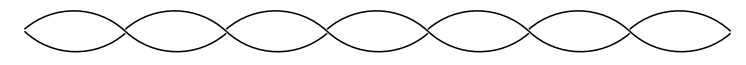
\includegraphics[scale=0.4]{./fig/joux.png}
\pause
Complexity: Running $\mathsf{A}$ for $t$ times. So expected complexity $t \times 2^{n/2}$
\end{frame}
\begin{frame}
	\frametitle{Cascaded Hash Function}
	\begin{block}{Cascading}
		\begin{enumerate}
		\item A natural way to build large hash values is to concatenate several smaller hashes.
		\item Consider two hash functions
		\begin{align*}
			\mathcal{F}:\{0,1\}^* \to \{0,1\}^n\\
			\mathcal{G}:\{0,1\}^* \to \{0,1\}^m
		\end{align*}
		Construct the cascaded hash $\h(x) = \mathcal{F}(x)\|\mathcal{G}(x)$
		\item What is the security of $\h$?
		\pause
		\item Output size of $\h$ is $(m+n)$, so using birthday attack the complexity will be $2^{\frac{m+n}{2}}$.
		\item \red{Can we do better?}
		\end{enumerate}
	\end{block}
\end{frame}
\begin{frame}
	\frametitle{Cascaded Hash Function}
	\begin{block}{Attack on Cascaded Hash Function}
		\begin{enumerate}
			\item Without the loss of generality, assume $n < m$.
			\item Using multi-collision idea, find $2^{m/2}$-multi-collisions on $\mathcal{F}$. The complexity of this step is \red{$\frac{m}{2}\times (2^{n/2})$}.
			\item Now we have $2^{m/2}$ messages with collision value, say $f$ on the $\mathcal{F}$ side.
		\end{enumerate}
	\end{block}
\pause
The hash values are of the form
\begin{align*}
	x_1 &\longrightarrow f\|g_1\\
	x_2 &\longrightarrow f\|g_2\\
	\vdots &\\
	x_{2^{m/2}} &\longrightarrow f\|g_{2^{m/2}}
\end{align*}
\end{frame}
\begin{frame}
	\frametitle{Cascaded Hash Function}
	\begin{block}{Attack on Cascaded Hash Function}
		\begin{enumerate}
			\item Now according to birthday paradox, these $2^{m/2}$ messages yields collision on the side of $\mathcal{G}$ also.
			\item We need \red{$2^{m/2}$} calls to $\mathcal{G}$.
			\item Total complexity \red{$\frac{m}{2}\times (2^{n/2}) + 2^{m/2}$}.
		\end{enumerate}
	\end{block}
\end{frame}

\begin{frame}
    \begin{center}
        {\huge {\color{red} Thank You} for your attention!} \\ \Large Any questions?
    \end{center}
\end{frame}

\bibliographystyle{alpha}
\bibliography{../bibliography.bib}

\end{document}
